\documentclass[12pt,a4paper]{article}
\usepackage{times}
\usepackage{durhampaper}
\usepackage{harvard}
\usepackage{url}
\citationmode{abbr}
\bibliographystyle{agsm}

\title{Cloud-based RAW image editing}
\author{Ryan Collins}
\supervisor{Dr Tom Friedetzky}
\student{Ryan Collins (gcdk35)}
\degree{M.Eng Computer Science}

\date{}

\begin{document}

\maketitle

\begin{abstract}
\paragraph{Context/Background}

\paragraph{Aims}
The main aim of this project is to test the feasibility of a Cloud-based RAW image
editor.
\paragraph{Method}
A render server backend will first be implemented as an API, taking in an input as a
JSON object, and then processing the image, and then a JavaScript
client shall be created to interface with this API.
\paragraph{Proposed Solution}
A web application that uses dcraw coupled with custom Java code to read RAW images,
and allow adjustment of various parameters, with the output being sent back to the user.
\end{abstract}

\begin{keywords}
RAW image editing, dcraw, cloud image editing
\end{keywords}

\section{Introduction}

% WHAT IS RAW? Why use RAW over JPEG
Many photographers use a file format (or rather, a family of very similar file formats) called RAW,
which rather than compressing the image and conducting some image manipulation on the camera,
store the RAW camera sensor data outputted by the camera sensor, for later processing and editing
by a computer. These files can be much larger than the compressed image, but provide a far greater
degree of control over the captured image, when compared with a compressed JPEG, along with an
increase in quality. A RAW file essentially acts as a digital negative, as the image can be edited
constantly without losing any quality between edits.  \cite{AllAboutTheFormat}

% Current software requires quite high specification machines to run. For simple tasks,
%  or for multiple users, getting access to these machines might be difficult/expensive.
%  Everyone has a web browser, so a web based RAW image editor would be ideal, allowing
%  access from mobile, tablets, or laptops.

% Furthermore, content management systems also require the processing of images. Currently,
%  photos are typically edited in a program like Photoshop/Lightroom, then they are exported
%  and uploaded to the CMS, where they are further processed by a CMS to reduce file sizes.
%  Instead of this, a Cloud service could be utilized to cut out the middle man, uploading RAW files
%  directly to the CMS, and then editing within a CMS itself.



\subsection{Project Aim}
The aim of this project is to produce a Cloud-based RAW image photo editor, both as an API (allowing potential
image rendering headlessly), along with a full RAW image editor interface via a web browser. The image photo editor
should be able to read at least DNG and NEF files, and allow contrast, colour and exposure adjustment, along with
noise reduction, haze removal, and auto correction options. Furthermore, this system should be multi-user, allowing more than
one user to edit RAW photos at a time through the web interface, each with their own individual collection of images.

\subsection{Deliverables}


\section{Design}

This section presents the proposed solutions of the problems in detail. The design details should all be placed in this section. You may create a number of subsections, each focusing on one issue.

This section should be up to 8 pages in length.
The rest of this section shows the formats of subsections as well as some general formatting information.  You should also consult the Word template.


\subsection{Requirements}



\subsection{Proposed Extensions}

\subsection{Architecture}
As the system is fairly large, it's important to break it down into individual pieces. These are:

\textbf{TODO: Add diagram of the system architecture}
  \subsubsection{Client Interface to Render Server Communication}
There are several options for communicating between the user interface and the render server.

\paragraph{Representational State Transfer (REST)}
A Representational State Transfer system would work by sending a request to the server,
requesting an image be rendered. This initial request will be replied to with a job number,
which will be quoted in further communications. From here, future requests will be made
over a regular interval, requesting the information for the specified job. If this job is finished,
the result will be returned, but otherwise further requests will need to be made. This is the process
of polling.

The XMLHttpRequest object in JavaScript, used to make AJAX requests, was designed by Microsoft
in 1999, and later adopted in the 2000s.
This method is definitely the most compatible with browsers, being compatible with Edge, Chrome,
Firefox, Internet Explorer 7+, Opera, and Safari. \cite{XMLHttpRequestMozilla}

However, this method does require making many requests and connections to the server,
coupled with code to regularly poll at an interval until done. While this will work, it's not the most
optimal solution, and the code produced from this would be more complex (code could be needed to issue jobs, recall jobs,
and to ensure that the person who requests the result of a job is actually allowed to see the result of the job).

\paragraph{Web Socket}
Web Socket allows for two way communication between a browser and a server. It acts in a similar
way to traditional TCP socket communication, only it incorporates the origin based security
model used within web browsers. By using web socket over REST, opening multiple HTTP connections
is not needed, as a single connection is maintained at all times. \cite{WebSocketProtocol}

\paragraph{Socket.io}
Socket.io is an implementation that relies on both REST and Web Socket.
If the browser supports web socket, then it is utilised, but in the event that the
user's browser does not support new web socket technologies, then it defaults to
using REST, and automatically polls regularly for information. This way, we get the
best of both options shown above, in such a way that the code itself remains fairly
tidy (as the polling nature of REST is abstracted away from our system).

\subsubsection{Render Server}
\textbf{TODO: ADD DIAGRAM OF THE RENDER SERVER SUB LAYERS (ADAMS, DCRAW)}
The render server takes instructions given to it (with accordance to our API), and
generates the output image based on the RAW image supplied, and the appropriate settings.

One of the first considerations is how to parse RAW files.

\paragraph{dcraw}
Dcraw is an executable that allows the processing of RAW image files.

Dcraw itself can then be used to convert to other formats, one being the uncompressed TIFF format,
giving us a very high quality image that can then be adjusted. Our system isn't merely a wrapper for
dcraw in this instance, but extends the features supplied by dcraw.
\textbf{TODO: Explain what DCRAW is, how it can be used.}
\textbf{TODO: DCRAW features, built in. Export as }
\paragraph{libraw}
LibRaw is a C++ library based on dcraw, that is designed as a library rather than just
an executable.

LibRaw would be used when loading RAW images, processing them, and then from this,
the image can be processed using custom routines (i.e. converting the libraw format
to a matrix representation, and then using that matrix representation to carry out
some manipulation).

While LibRaw has many useful features, the documentation is somewhat limited.

\paragraph{ImageMagick}
ImageMagick is a library that can be used to process any images, not just RAW. While it can read
RAW image files, it also has many more features, including many feature that we don't need/want to
implement ourselves for the purpose of this project. As such, I believe while ImageMagick is a good option,
it's a bit too heavy for our use.
\textbf{TODO: SOURCE FOR IMAGEMAGICK READING RAW FILES}
\textbf{TODO: SOURCE FOR FEATURES OF IMAGE MAGICK}

\subsubsection{Client-side Interface}
  The page design of the interface shall follow the design in \ref{UserInterface}.
  The goal of the client side interface is to allow adjustment of the image parameters,
  and show a preview whenever a parameter is changed.

  To display the image, an HTML5 Canvas will provide a large amount of control to
  how we can display the image, allowing for features such as zooming, and drawing. This can't be
  achieved using a standard HTML image.

\subsection{User Interface}\label{UserInterface}
  A sidebar should be used as the main interface for adjusting image parameters.
  This sidebar should be able to be hidden, showing the image fully underneath.
  When the sidebar is in the expanded state, the preview image should be displayed
  fully on screen.

  The user interface design is shown in Figure \ref{UXDesign1}

  Within the sidebar, clicking on a navigation item will display a new submenu.
  If the item is a parameter adjustment, updating the value in the menu will also
  update the value that is sent to the render server to generate a preview.

\textbf{TODO ADD INTERFACE DRAWINGS.}
  % \begin{figure}[h]
  %   \caption{The editor interface, with the sidebar expanded.}
  %   \centering
  %   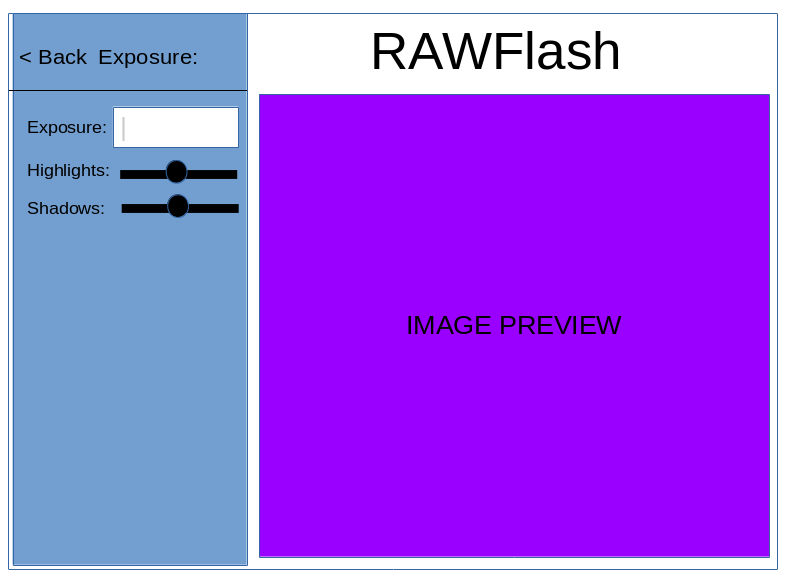
\includegraphics[width=0.5\textwidth]{uxdesign1}
  % \end{figure}

\subsection{Implementation Information}
Each individual module of the system requires different technologies in order to
produce an overall system.

\paragraph{Client-side Interface}
For this, HTML5, CSS3 and JavaScript (with jQuery to provide extra functionality)
are ideal, as HTML5 can be used to create the user interface, with CSS3 providing styling
and some basic animation to improve the UX. Using JavaScript with jQuery, it allows us
to keep track of the state of the editor, and transmit and receive information between client and
render server with help of some library. jQuery is useful for interfacing with the
DOM (the webpage itself, and it's components), allowing us to specify events, and functions
to run on particular events, along with template loading and various other functionalities.

As this is mostly static content, and doesn't directly require any web service to be
performed for the main editor, the static content can be hosted using a web server like
Apache or NGINX, only serving static content, without any dynamic scripting needed.

NGINX is what I'd recommend in this situation because unlike Apache, NGINX isn't
configured out of the box for dynamic content (e.g. PHP/Python/other external processor).
As we don't need any dynamic content, as we are just serving static files, NGINX is ideal
for our workload (as less overhead is needed for features that won't be used such as
dynamic content rendered on the server side). \cite{ApacheVSNGINX}

\paragraph{Render Server}
While lower level programming languages might be useful for image processing,
the requirement of linking this with web technologies means that a language such as C
or C++ is not as ideal.

Java is a better choice, as there are libraries available to provide web services (REST),
along with Web Socket implementations, along with Socket IO. Furthermore, Java contains
some libraries within the language that allow for image manipulation, most notably
BufferedImage related features such as ConvolveOp, image resizing, and various other standard
features build in. This is useful, as rather than starting completely from scratch, the custom
image processing routines can build on the built in Java implementations, and create more advanced
algorithms using them.

While Java doesn't support loading TIFF into BufferedReader using ImageIO directly,
an extension exists online, in the form of TwelveMonkeys. No RAW image loading library
exists within Java, but an executable such as dcraw or rawspeed can be used to generate a file
that can be read within Java, while retaining the quality (e.g. uncompressed TIFF). This can be done
using ProcessBuilder, and ideally writing a library to do this.
% of course, this library became jdcraw.

As this system will likely use a large amount of external dependencies, a dependency management tool
like Apache Maven should be used, to both manage dependencies from an external source (e.g. GitHub, Maven
Repositories), and also to build the system.
\textbf{TODO: reference libraries here.}

\paragraph{Account Management Server}
As this system needs to be used by multiple people, we need to have some record of users,
and their associated images.

Rather than rendering each page dynamically, we can instead use JavaScript to make AJAX requests,
fetching the data needed, and this way, we don't need to render whole HTML web pages. In terms of
backend technology, it doesn't matter too much what is used, as it won't be used too much, but
in my case I'll be using Node.JS with an Express server, simply because it's easy to deploy and
install dependencies ("npm install" can be run to install dependencies in one command), and it can
also connect to a database to provide services such as login, and records of individual files.

\paragraph{Distributed System Management}
As this system consists of several smaller systems, it's important that these are
managed. For each smaller component, a Docker container can be created, containing the
configuration between each one. From here, Docker Compose can then be used to manage
the entire system, bringing everything online, opening ports, and building everything
automatically.

This requires us to create a Dockerfile per system (one for the render server,
one for the client front-end). This Dockerfile specifies the image to build from,
along with instructions that need to be run, and files that should be shared, to make
that container work. Rather than customising an individual image, this customisation can be done
by building on existing images, saving time without needing to start again from scratch. \cite{DockerWhyItsUseful}

\textbf{TODO: some source of docker}
\subsection{Evaluation}
% \subsection{Main Text}
%
% The font used for the main text should be Times New Roman (Times) and the font size should be 12.  The first line of all paragraphs should be indented by 0.25in, except for the first paragraph of each section, subsection, subsubsection etc. (the paragraph immediately after the header) where no indentation is needed.
%
% \subsection{Figures and Tables}
% In general, figures and tables should not appear before they are cited.  Place figure captions below the figures; place table titles above the tables.  If your figure has two parts, for example, include the labels ``(a)'' and ``(b)'' as part of the artwork.  Please verify that figures and tables you mention in the text actually exist.  make sure that all tables and figures are numbered as shown in Table \ref{units} and Figure 1.
% %sort out your own preferred means of inserting figures
%
% \begin{table}[htb]
% \centering
% \caption{UNITS FOR MAGNETIC PROPERTIES}
% \vspace*{6pt}
% \label{units}
% \begin{tabular}{ccc}\hline\hline
% Symbol & Quantity & Conversion from Gaussian \\ \hline
% \end{tabular}
% \end{table}

\section{References}

% The list of cited references should appear at the end of the report, ordered alphabetically by the surnames of the first authors.  The default style for references cited in the main text is the  Harvard (author, date) format.  When citing a section in a book, please give the relevant page numbers, as in \cite[p293]{budgen}.  When citing, where there are either one or two authors, use the names, but if there are more than two, give the first one and use ``et al.'' as in  , except where this would be ambiguous, in which case use all author names.
%
% You need to give all authors' names in each reference.  Do not use ``et al.'' unless there are more than five authors.  Papers that have not been published should be cited as ``unpublished'' \cite{euther}.  Papers that have been submitted or accepted for publication should be cited as ``submitted for publication'' as in \cite{futher} .  You can also cite using just the year when the author's name appears in the text, as in ``but according to Futher \citeyear{futher}, we \dots''.  Where an authors has more than one publication in a year, add `a', `b' etc. after the year.

\bibliography{report}


\end{document}
